\section{Дерево отрезков}
\textbf{Дерево отрезков} (англ. Segment tree)~--- это структура данных, которая позволяет за асимптотику $O(logN)$
реализовать любые операции, определяемые на множестве, на котором данная операция ассоциативна,
и существует нейтральный элемент относительно этой операции, то есть на моноиде.

Например, суммирование на множестве натуральных чисел, поиск минимума на любом числовом множестве,
перемножение матриц на множестве матриц размера $N \times N$, объединение множеств,
поиск наибольшего общего делителя на множестве целых чисел и многочленов.

При этом дополнительно возможно изменение элементов массива: как изменение значения одного элемента,
так и изменение элементов на целом подотрезке массива, например разрешается присвоить всем элементам $a[l..r]$ какое-либо значение,
либо прибавить ко всем элементам массива какое-либо число.
Структура занимает $O(n)$ памяти, а ее построение требует $O(n)$ времени.

\subsection{Построение дерева}
Пусть исходный массив a состоит из $n$ элементов.
Для удобства построения увеличим длину массива a так, чтобы она равнялась ближайшей степени двойки, т.е. $2^k$, где $2^k \ge n$.
Это сделано, для того чтобы не допустить обращение к несуществующим элементам массива при дальнейшем процессе построения.
Пустые элементы необходимо заполнить нейтральными элементами моноида.
Тогда для хранения дерева отрезков понадобится массив $t$ из $2^{k+1}$ элементов,
поскольку в худшем случае количество вершин в дереве можно оценить суммой $n+\frac{n}{2}+\frac{n}{4}+\ldots+1 < 2n$, где $n=2^k$.
Таким образом, структура занимает линейную память.

Процесс построения дерева заключается в заполнении массива $t$.
Заполним этот массив таким образом, чтобы $i$-й элемент являлся бы результатом некоторой бинарной операции
(для каждой конкретной задачи своей) от элементов c номерами $2i+1$ и $2i+2$,
то есть родитель являлся результатом бинарной операции от своих сыновей (обозначим в коде эту операцию как \texttt{OP}).
Один из вариантов~--- делать рекурсивно.
Пусть у нас имеются исходный массив a, а также переменные $tl$ и $tr$, обозначающие границы текущего полуинтервала.
Запускаем процедуру построения от корня дерева отрезков ($i=0$, $tl=0$, $tr=n$), а сама процедура построения,
если её вызвали не от листа, вызывает себя от каждого из двух сыновей и суммирует вычисленные значения,
а если её вызвали от листа~--- то просто записывает в себя значение этого элемента массива (Для этого у нас есть исходный массив a).
Асимптотика построения дерева отрезков составит, таким образом, $O(n)$.

Выделяют два основных способа построения дерева отрезков: построение снизу и построение сверху.
При построении снизу алгоритм поднимается от листьев к корню
(Просто начинаем заполнять элементы массива $t$ от большего индекса к меньшему, таким образом при заполнении элемента $i$ его дети
$2i+1$ и $2i+2$ уже будут заполнены, и мы с легкостью посчитаем бинарную операцию от них),
а при построении сверху спускается от корня к листьям.
Особенные изменения появляются в реализации запросов к таким деревьям отрезков.

\begin{figure}
\centering
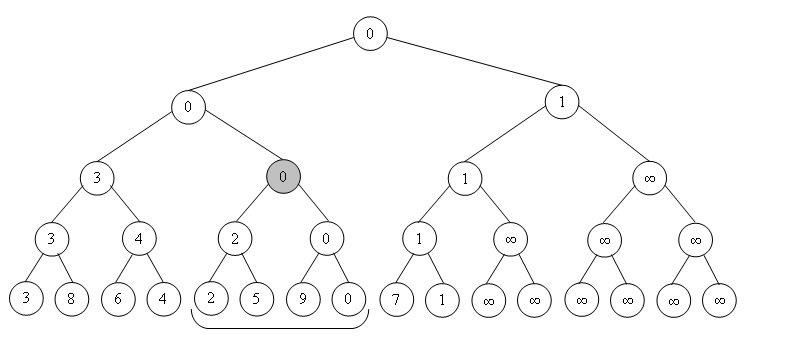
\includegraphics[scale=0.5]{images/SegmentTree.jpg}
\caption{Дерево отрезков}
\label{fig:segment_tree}
\end{figure}

\subsection{Реализация запроса в дереве отрезков сверху}

Данная операция позволяет выполнять запросы на дереве отрезков, причем алгоритм запускается от корня и рекурсивно идет сверху вниз.

\textbf{Алгоритм}

\textit{Замечание}. Используем в алгоритме не отрезки, а полуинтервалы (левая граница включительно, а правая — нет).

Пусть есть уже построенное дерево отрезков и идет запрос на полуинтервале $[a \ldots b)$.

В качестве параметров рекурсий передаем следующие переменные:
\begin{itemize}
    \item $node$ — номер (в массиве с деревом отрезков) текущей вершины дерева.
    \item $a$, $b$ — левая и правая границы запрашиваемого полуинтервала.
\end{itemize}

Пусть $l$, $r$ — это левая и правая границы полуинтервала, за которые <<отвечает>> наша вершина. Запустим рекурсивную процедуру от всего полуинтервала (то есть от корневой вершины).

Для текущего состояния проверяем следующие условия :
\begin{itemize}
    \item Если текущий полуинтервал не пересекается с искомым, то возвращаем нейтральный элемент.
    \textit{Например}: текущий [1…3), а искомый [3…5).
    \item Если текущий полуинтервал лежит внутри запрашиваемого полуинтервала, то возвращаем значение в текущей вершине.
    \textit{Например}: текущий [2…3), а искомый [2…4).
    \item Иначе переходим к рекурсивным вызовам функций от детей вершины. При этом возвращаем значение на текущем полуинтервале, как функцию (соответствующую типу нашего запроса) от результатов выполнения на детях.
\end{itemize}

\begin{figure}
\centering
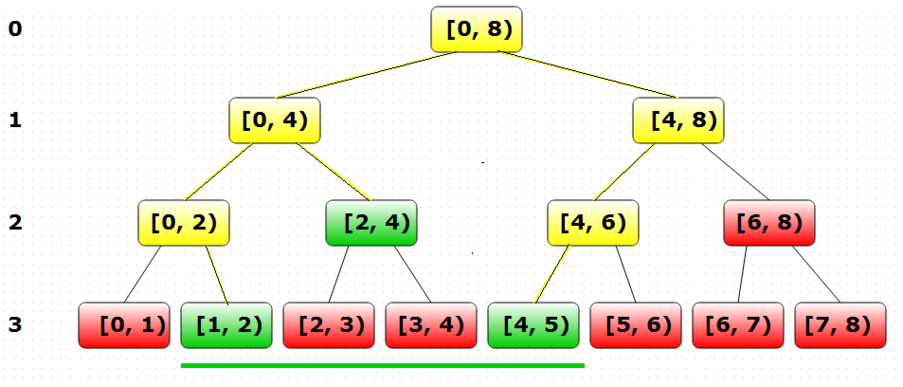
\includegraphics[scale=0.7]{images/SegmentTreeQueryTB.png}
\caption{Дерево отрезков. Интервальный запрос}
\label{fig:segment_tree_interval}
\end{figure}

Так как на каждом уровне дерева рекурсия может дойти до не более, чем двух вершин (иначе бы нашлось две рядом стоящие вершины одного уровня, объединение которых дало отрезок, за который отвечает вершина предыдущего уровня), а всего уровней $\log n$, то операция выполняется за $O(\log n)$.

\subsection{Примеры использования дерева отрезков}

\subsubsection{Поиск минимума/максимума}

Немного изменим условие задачи: будем производить запрос минимума/максимума на отрезке.

Тогда в дереве отрезков надо изменить способ вычисления пометки во внутренних вершинах: использовать минимум/максимум из пометок сынове. По сути пометка вершины дерева будет равна минимальному/максимальному элемент на всем отрезке, за который отвечает вершины дерева.

\subsubsection{Поиск минимума/максимума и количества раз, которое он встречается}

Задача аналогична предыдущей, только теперь помимо минимума/максимума требуется также возвращать количество его вхождений. Эта задача встаёт естественным образом, например, при решении с помощью дерева отрезков такой задачи: найти количество наидлиннейших возрастающих подпоследовательностей в заданном массиве.

Для решения этой задачи в каждой вершине дерева отрезков будем хранить пару чисел: кроме минимума/максимума количество его вхождений на соответствующем отрезке. Тогда при построении дерева мы должны просто по двум таким парам, полученным от сыновей текущей вершины, получать пару для текущей вершины.

Объединение двух таких пар в одну стоит выделить в отдельную функцию, поскольку эту операцию надо будет производить и в запросе модификации, и в запросе поиска минимума/максимума.

\subsubsection{Поиск наибольшего общего делителя / наименьшего общего кратного}
Т.е. мы хотим научиться искать НОД/НОК всех чисел в заданном отрезке массива.

Это довольно интересное обобщение дерева отрезков получается абсолютно таким же путём, как и деревья отрезков для суммы/минимума/максимума: достаточно просто хранить в каждой вершине дерева НОД/НОК всех чисел в соответствующем отрезке массива.

Обратим внимание, что в каждой вершине при обновлении информации нужно будет выполнить более сложную операцию -- вычисление наибольшего общего делителя пометок сыновей.

\subsubsection{Подсчёт количества нулей, поиск $k$-го нуля}

Мы хотим научиться отвечать на запрос количества нулей в заданном отрезке массива, а также на запрос нахождения $k$-го нулевого элемента.

Снова немного изменим данные, хранящиеся в дереве отрезков: будем хранить теперь в пометке вершины количество нулей, встречающихся в соответствующих отрезках массива. Понятно, как поддерживать и использовать эти данные в функциях построения дерева, обновления элемента и запроса — тем самым мы решили задачу о количестве нулей в заданном отрезке массива.

Теперь научимся решать задачу о поиске позиции $k$-го вхождения нуля в массиве. Для этого будем спускаться по дереву отрезков, начиная с корня, и переходя каждый раз в левого или правого сына в зависимости от того, в каком из отрезков находится искомый $k$-ый ноль. В самом деле, чтобы понять, в какого сына нам надо переходить, достаточно посмотреть на значение, записанное в левом сыне: если оно больше либо равно $k$, то переходить надо в левого сына (потому что в его отрезке есть как минимум $k$ нулей), а иначе — переходить в правого сына.

При реализации можно отсечь случай, когда $k$-го нуля не существует, ещё при входе в функцию, вернув в качестве ответа, например, -1.

\subsubsection{Поиск префикса массива с заданной суммой}
Мы хотим по данному значению $x$ быстро найти такое $i$, что сумма первых $i$ элементов массива $a$ больше либо равна $x$ (считая, что массив $a$ содержит только неотрицательные числа).

Эту задачу можно решать бинарным поиском, вычисляя каждый раз внутри него сумму на том или ином префиксе массива, но это приведёт к решению за время $O (\log^2 n)$.

Вместо этого можно воспользоваться той же самой идеей, что и в предыдущем пункте, и искать искомую позицию одним спуском по дереву: переходя каждый раз в левого или правого сына в зависимости от величины суммы в левом сыне. Тогда ответ на запрос поиска будет представлять собой один такой спуск по дереву, а, следовательно, будет выполняться за $O (\log n)$.

\subsubsection{Поиск подотрезка с максимальной суммой}
По-прежнему на вход даётся массив $a$, и поступают запросы $(l,r)$, которые означают: найти такой подотрезок $a[l^\prime \ldots r^\prime]$, что $l \le l^\prime, r^\prime \le r$, и сумма этого отрезка $a[l^\prime \ldots r^\prime]$ максимальна. Запросы модификации отдельных элементов массива допускаются. Элементы массива могут быть отрицательными (и, например, если все числа отрицательны, то оптимальным подотрезком будет пустой — на нём сумма равна нулю).

Это весьма нетривиальное обобщение дерева отрезков получается следующим образом. Будем хранить в каждой вершине дерева отрезков четыре величины: сумму на этом отрезке, максимальную сумму среди всех префиксов этого отрезка, максимальную сумму среди всех суффиксов, а также максимальную сумму подотрезка на нём. Иными словами, для каждого отрезка дерева отрезков ответ на нём уже предпосчитан, а также дополнительно ответ посчитан среди всех отрезков, упирающихся в левую границу отрезка, а также среди всех отрезков, упирающихся в правую границу.

Подойдём к этому с рекурсивной точки зрения: пусть для текущей вершины все четыре значения в левом сыне и в правом сыне уже подсчитаны, посчитаем их теперь для самой вершины. Заметим, что ответ в самой вершине равен:
\begin{itemize}
    \item либо ответу в левом сыне, что означает, что лучший подотрезок в текущей вершине целиком помещается в отрезок левого сына,
    \item либо ответу в правом сыне, что означает, что лучший подотрезок в текущей вершине целиком помещается в отрезок правого сына,
    \item либо сумме максимального суффикса в левом сыне и максимального префикса в правом сыне, что означает, что лучший подотрезок лежит своим началом в левом сыне, а концом — в правом.
\end{itemize}

Значит, ответ в текущей вершине равен максимуму из этих трёх величин. Пересчитывать же максимальную сумму на префиксах и суффиксах совсем несложно. Необходимо аккуратно рассмотреть случаи, когда левый/правый сын целиком входит в префикс или суффикс.

Осталось разобраться с ответом на запрос. Для этого мы так же, как и раньше, спускаемся по дереву, разбивая тем самым отрезок запроса $[l \ldots r]$ на несколько подотрезков, совпадающих с отрезками дерева отрезков, и объединяем ответы в них в единый ответ на всю задачу. Тогда понятно, что работа ничем не отличается от работы обычного дерева отрезков, только надо вместо простого суммирования/минимума/максимума значений использовать функцию комбинирования информации, описанной выше.

\subsection{Сохранение всего подмассива в каждой вершине дерева отрезков}

Это отдельный подраздел, стоящий особняком от остальных, поскольку в каждой вершине дерева отрезков мы будем хранить не какую-то сжатую информацию об этом подотрезке (сумму, минимум, максимум и т.п.), а все элементы массива, лежащие в этом подотрезке. Таким образом, корень дерева отрезков будет хранить все элементы массива, левый сын корня — первую половину массива, правый сын корня — вторую половину, и так далее.

Самый простой вариант применения этой техники — когда в каждой вершине дерева отрезков хранится отсортированный список всех чисел, встречающихся в соответствующем отрезке. В более сложных вариантах хранятся не списки, а какие-либо структуры данных, построенные над этими списками (\rm set, \rm map и т.д.). Но все эти методы объединяет то, что в каждой вершине дерева отрезков хранится некая структура данных, имеющая в памяти размер порядка длины соответствующего отрезка.

Первый естественный вопрос, встающий при рассмотрении деревьев отрезков этого класса — это объём потребляемой памяти. Утверждается, что если в каждой вершине дерева отрезков хранится список всех встречающихся на этом отрезке чисел, либо любая другая структура данных размера того же порядка, то в сумме всё дерево отрезков будет занимать $O (n \log n)$ ячеек памяти. Потому что каждое число $a[i]$ попадает в $O (\log n)$ отрезков дерева отрезков (хотя бы потому, что высота дерева отрезков есть $O (\log n))$, а на каждом уровне дерева число встречается ровно один раз.

Итак, несмотря на кажущуюся расточительность такого дерева отрезков, оно потребляет памяти не сильно больше обычного дерева отрезков.

Рассмотрим несколько типичных применений такой структуры данных.

\subsubsection{Поиск наименьшего числа, больше либо равного заданного, в указанном отрезке. Запросов модификации нет}

Требуется отвечать на запросы следующего вида: $(l,r,x)$, что означает найти минимальное число в отрезке $a[l \ldots r]$, которое больше либо равно $x$.

Построим дерево отрезков, в котором в каждой вершине будем хранить отсортированный список всех чисел, встречающихся на соответствующем отрезке. Например, корень будет содержать массив $a$ в отсортированном виде. Для построения такого дерева подойдём к задаче, как обычно, с точки зрения рекурсии: пусть для левого и правого сыновей текущей вершины эти списки уже построены, и нам требуется построить этот список для текущей вершины. При такой постановке вопроса становится почти очевидно, что это можно сделать за линейное время: нам просто надо объединить два отсортированных списка в один, что делается одним проходом по ним с двумя указателями (операция слияния из сортировки слиянием).

Построенное таким образом дерево отрезков будет занимать $O (n \log n)$ памяти. А благодаря такой реализации время его построения также есть величина $O (n \log n)$ — ведь каждый список строится за линейное относительно его размера время. (Кстати говоря, здесь прослеживается очевидная аналогия с алгоритмом сортировки слиянием: только здесь мы сохраняем информацию со всех этапов работы алгоритма, а не только итог.)

Теперь рассмотрим ответ на запрос. Будем спускаться по дереву, как это делает стандартный ответ на запрос в дереве отрезков, разбивая наш отрезок $a[l \ldots r]$ на несколько подотрезков (порядка $O (\log n)$ штук). Понятно, что ответ на всю задачу равен минимуму среди ответов на каждом из этих подотрезков. Поймём теперь, как отвечать на запрос на одном таком подотрезке, совпадающем с некоторой вершиной дерева.

Итак, мы пришли в какую-то вершину дерева отрезков и хотим посчитать ответ на ней, т.е. найти минимальное число, больше либо равное данного x. Для этого нам всего лишь надо выполнить бинарный поиск по списку, посчитанному в этой вершине дерева, и вернуть первое число из этого списка, больше либо равное x.

Таким образом, ответ на запрос в одном подотрезке происходит за $O (\log n)$, а весь запрос обрабатывается за время $O (\log^2 n)$.

\subsubsection{Поиск наименьшего числа, больше либо равного заданного, в указанном отрезке. Допускаются запросы модификации}

Задача аналогична предыдущей, только теперь разрешены запросы модификации: обработать присвоение $a[i] = y$.

Решение также аналогично решению предыдущей задачи, только вместо простых списков в каждой вершине дерева отрезков мы будем хранить сбалансированный список, который позволяет быстро искать требуемое число, удалять его, а также вставлять новое число. Учитывая, что вообще говоря число во входном массиве могут повторяться, оптимальным выбором является структура данных \rm multiset.

Построение такого дерева отрезков происходит примерно так же, как и в предыдущей задаче, только теперь надо объединять не отсортированные списки, а \rm multiset, что приведёт к тому, что асимптотика построения ухудшится до $O (n \log^2 n)$.

Ответ на запрос поиска вообще практически эквивалентен приведённому случаю, только теперь lower\_bound нужно искать в multiset (вершинах из рабиения отрезка на элементарные).

Наконец, запрос модификации. Для его обработки мы должны спуститься по дереву, внеся изменения во все $O (\log n)$ списков, содержащих затрагиваемый элемент. Мы просто удаляем старое значение этого элемента (не забыв, что нам не надо удалить вместе с ним все повторы этого числа) и вставляем его новое значение.

Обработка этого запроса происходит также за время $O (\log^2 n)$.

\subsection{Обновление на отрезке}
Выше рассматривались только задачи, когда запрос модификации затрагивает единственный элемент массива. На самом деле, дерево отрезков позволяет делать запросы, которые применяются к целым отрезкам подряд идущих элементов, причём выполнять эти запросы за то же время $O (\log n)$.

\subsubsection{Прибавление на отрезке}
Начнём рассмотрение деревьев отрезков такого рода с самого простого случая: запрос модификации представляет собой прибавление ко всем числам на некотором подотрезке $a[l \ldots r]$ некоторого числа $x$. Запрос чтения — по-прежнему считывание значения некоторого числа $a[i]$.

Чтобы делать запрос прибавления эффективно, будем хранить в каждой вершине дерева отрезков, сколько надо прибавить ко всем числам этого отрезка целиком. Например, если приходит запрос <<прибавить ко всему массиву  $a[0 \ldots n-1]$ число 2>>, то мы поставим в корне дерева число 2. Тем самым мы сможем обрабатывать запрос прибавления на любом подотрезке эффективно, вместо того чтобы изменять все $O (n)$ значений.

Если теперь приходит запрос чтения значения того или иного числа, то нам достаточно спуститься по дереву, просуммировав все встреченные по пути значения, записанные в вершинах дерева.

\subsubsection{Присвоение на отрезке}
Пусть теперь запрос модификации представляет собой присвоение всем элементам некоторого отрезка $a[l \ldots r]$ некоторого значения $p$. В качестве второго запроса будем рассматривать считывание значения массива $a[i]$.

Чтобы делать модификацию на целом отрезке, придётся в каждой вершине дерева отрезков хранить, покрашен ли этот отрезок целиком в какое-либо число или нет (и если покрашен, то хранить само это число). Это позволит нам делать <<запаздывающее>> обновление дерева отрезков: при запросе модификации мы, вместо того чтобы менять значения во множестве вершин дерева отрезков, поменяем только некоторые из них, оставив флаги <<покрашен>> для других отрезков, что означает, что весь этот отрезок вместе со своими подотрезками должен быть покрашен в этот цвет.

Итак, после выполнения запроса модификации дерево отрезков становится, вообще говоря, неактуальным — в нём остались недовыполненными некоторые модификации.

Например, если пришёл запрос модификации <<присвоить всему массиву $a[0 \ldots n-1]$ какое-то число>>, то в дереве отрезков мы сделаем единственное изменение — пометим корень дерева, что он покрашен целиком в это число. Остальные же вершины дерева останутся неизменёнными, хотя на самом деле всё дерево должно быть покрашено в одно и то же число.

Предположим теперь, что в том же дереве отрезков пришёл второй запрос модификации — покрасить первую половину массива $a[0 \ldots n/2]$ в какое-либо другое число. Чтобы обработать такой запрос, мы должны покрасить целиком левого сына корня в этот новый цвет, однако перед тем как сделать это, мы должны разобраться с корнем дерева. Тонкость здесь в том, что в дереве должно сохраниться, что правая половина покрашена в старый цвет, а в данный момент в дереве никакой информации для правой половины не сохранено.

Выход таков: произвести проталкивание информации из корня, т.е. если корень дерева был покрашен в какое-либо число, то покрасить в это число его правого и левого сына, а из корня эту отметку убрать. После этого мы можем спокойно красить левого сына корня, не теряя никакой нужной информации.

Обобщая, получаем: при любых запросах с таким деревом (запрос модификации или чтения) во время спуска по дереву мы всегда должны делать проталкивание информации из текущей вершины в обоих её сыновей. Можно понимать это так, что при спуске по дереву мы применяем запаздывающие модификации, но ровно настолько, насколько это необходимо (чтобы не ухудшить асимптотику с $O (\log n)$).

При реализации это означает, что нам надо сделать функцию, которой будет передаваться вершина дерева отрезков, и она будет производить проталкивание информации из этой вершины в обоих её сыновей. Вызывать эту функцию следует в самом начале функций обработки запросов (но не вызывать её из листьев, ведь из листа проталкивать информацию не надо, да и некуда).

Для получения значения элемента $a[i]$ будет искать самую высокую <<покрашеную>> вершину на пути к элементу, или возьмем само значение элемента, если покрашеных вершин нет.

\subsubsection{Прибавление на отрезке, запрос максимума}
Запросом модификации снова будет запрос прибавления ко всем числам некоторого подотрезка одного и того же числа, а запросом чтения будет нахождение максимума в некотором подотрезке.

Тогда в каждой вершине дерева отрезков надо будет дополнительно хранить максимум на всём этом подотрезке. Но тонкость здесь заключается в том, как надо пересчитывать эти значения.

Например, пусть произошёл запрос <<прибавить ко всей первой половине, т.е. $a[0 \ldots n/2]$, число 2>>. Тогда в дереве это отразится записью числа 2 в левого сына корня. Как теперь посчитать новое значение максимума в левом сыне и в корне? Здесь становится важно не запутаться — какой максимум хранится в вершине дерева: максимум без учёта прибавления на всей этой вершине, или же с учётом его. Выбрать можно любой из этих подходов, но главное — последовательно использовать его везде. Например, при первом подходе максимум в корне будет получаться как максимум из двух чисел: максимум в левом сыне плюс прибавление в левом сыне, и максимум в правом сыне плюс прибавление в нём. При втором же подходе максимум в корне будет получаться как прибавление в корне плюс максимум из максимумов в левом и правом сыновьях, но прибавление на отрезке кроме изменения поментки добавленной суммы будет изменять и максимум на отрезке.

\subsection{Задания по теме}
\subsubsection{Теоретическое задание}
В решении этой задачи необходимо использовать Дерево отрезков
\textbf{без интервальной модификации}.

Опишите алгоритм решения следующей задачи.
Перед вами полоска длины $N$, разбитая на $N$ одинаковых квадратиков, пронумерованных слева направо числами от 0 до $N-1$. За одну операцию изменения (метод, предоставляемый интерфейсом вашей структуры данных) вы должны перекрасить все клетки с номерами от $L$ до $R$ включительно:
белые должны стать черными, а черные - белыми. В запросах поиска необходимо определить цвет клетки в позиции $X$. Изначально задается раскраска полоски в черный и белый цвет.

Интерфейс:
\begin{verbatim}
        Init(vector colors);
        ChangeColor(L, R);
        GetColor(X).
\end{verbatim}

Время работы метода Init должно быть линейным, а методов ChangeColor и GetColor должно быть $O(\log N)$.

\subsubsection{Практическое задание}
Задан массив $A$ из $n$ положительных чисел $a_{i} (1 \le a_{i} \le 10^9)$. Необходимо уметь выполнять 4 вида запросов:
\begin{itemize}
    \item 1 $p$ $v$ — присвоить $p$-му элементу массива значение $v$.
    \item 2 $l$ $r$ ($l \le r$) — прибавить единицу ко всем числам на отрезке $[l..r]$.
    \item 3 $l$ $r$ ($l \le r$) — найти сумму четных чисел на отрезке $[l..r]$.
    \item 4 $l$ $r$ ($l \le r$) — найти сумму нечетных чисел на отрезке $[l..r]$.
\end{itemize}
